\documentclass[twocolumn]{article}

\usepackage[unicode=true]{hyperref}
\usepackage{enumitem}
\usepackage{graphicx,grffile}

\title{\textbf{Autoreduction - an automated data reduction system for beam instruments}}
\author{J. R. Corderoy\\
ISIS Facility, Rutherford Appleton Laboratory\\
Email: jrc91@cam.ac.uk}
\date{23/09/2015}

\begin{document}
\maketitle

\subsection*{Abstract}\label{abstract}

A key step for users of large research facilities is the routine
processing of instrument data before use. Autoreduction is a software
system designed to automate this process, integrated with other
pre-existing facility systems and software packages, and provide
an interface for users to control it.

\section{Introduction}\label{introduction}

High-energy particle facilities, such as the ISIS Neutron and Muon
Facility, allow users in academic and industrial research
to perform experiments using instruments set up to use high-energy
particle beams. Common to most instruments is the need to process -- 
`reduce' -- raw data collected from an instrument into a usable dataset.

The goal for the autoreduction system is to provide a useful automation
step in this process. It allows data coming off an instrument to be
automatically reduced using a dedicated software package such as 
Mantid\cite{mantid}, while lending transparency to the process and
letting users control it through a straightforward web interface.

Presented below is an overview of the motivation and design of the system,
its use and interface, and its current status in production at ISIS.

\section{Background}\label{background}

\subsection{Usage}\label{usage}

This system was originally designed for use at the Spallation Neutron
Source at Oak Ridge National Laboratory, then subsequently at the ISIS
neutron source of the Science and Technology Facilities Council. These
facilities operate pulsed neutron sources for scientific and industrial
research, with many independent instruments receiving neutrons from a
source for use in experiments.

In both cases autoreduction was intended to serve as part of an
automation system to handle data produced by these neutron beam
instruments. However, the process is applicable to beamline instruments
in general, such as might be used on muon or X-ray beams.

\subsection{Data reduction}\label{data-reduction}

The autoreduction service exists to reduce beamline instrument data. An
instrument produces discrete tranches of data, referred to as `runs', in
service of experiments. This raw data typically needs to be processed --
`reduced' -- before it can be used by scientists, by running a script on
it. Although the script itself need not change often, it may have
configurable parameters -- variables -- which ought to be changed
frequently.

The autoreduction system is intended to automate this process.
Instrument scientists provide it with reduction scripts - in a specified
location on a shared file archive - and sets of variables to use to
reduce runs. The system watches for the completion of runs, and runs the
appropriate script, with the correct variables, on them, supplying the
reduced data to an archive for users to retrieve.

\subsection{Requirements}\label{requirements}

The system is intended primarily to serve the instrument scientists --
who manage beamline instruments -- and users who use the instruments to
run experiments. The key requirements for these users were to

\begin{enumerate}[noitemsep]
\item
  Automate the reduction of data from beam instruments, using scripts
  provided by instrument scientists.
\item
  Show the status of reduction on runs, as well as the results and
  locations of reduced data, to users.
\item
  Allow instrument scientists to set the parameters used for reduction,
  in advance and retroactively.
\item
  Allow users and instrument scientists to see what script, with which
  parameters, was used to reduce a run.
\item
  Allow users and instrument scientists to modify the parameters used
  for a run, and re-run reduction using new parameters or scripts.
\end{enumerate}

Additional constraints were to

\begin{enumerate}[noitemsep,resume]
\item
  Limit access to the system to ensure that only staff and scientists
  can access runs and instruments.
\item
  Utilise existing authentication systems to validate identities and
  permissions for (1).
\item
  Allow scalability for processing large amounts of data in a timely
  manner.
\item
  Integrate with ICAT\cite{icat} -- the scientific metadata catalogue in use
  at ISIS.
\end{enumerate}

\section{System architecture}\label{system-architecture}

The architecture is based on a queue node, which co-ordinates
communication between all components of the system. This maintains
separate message queues, which allow components to act on messages from
other components and update the system. These components are

\begin{itemize}[noitemsep]
\item
  A listener for new jobs
\item
  The state database \& coordinator
\item
  Workers for reduction processing
\end{itemize}

When the listener detects that a new job should be created, it sends a
request to do so to \emph{Data Ready}. The state database consumes the
request and creates the corresponding job in the database, before
sending a request to process it to \emph{Reduction Pending}. A reduction
worker takes this message and runs the appropriate script, sending the
result to either \emph{Reduction Complete} or \emph{Reduction Error},
where it's consumed by the state database to update the status of the
run.

\begin{figure*}
\centering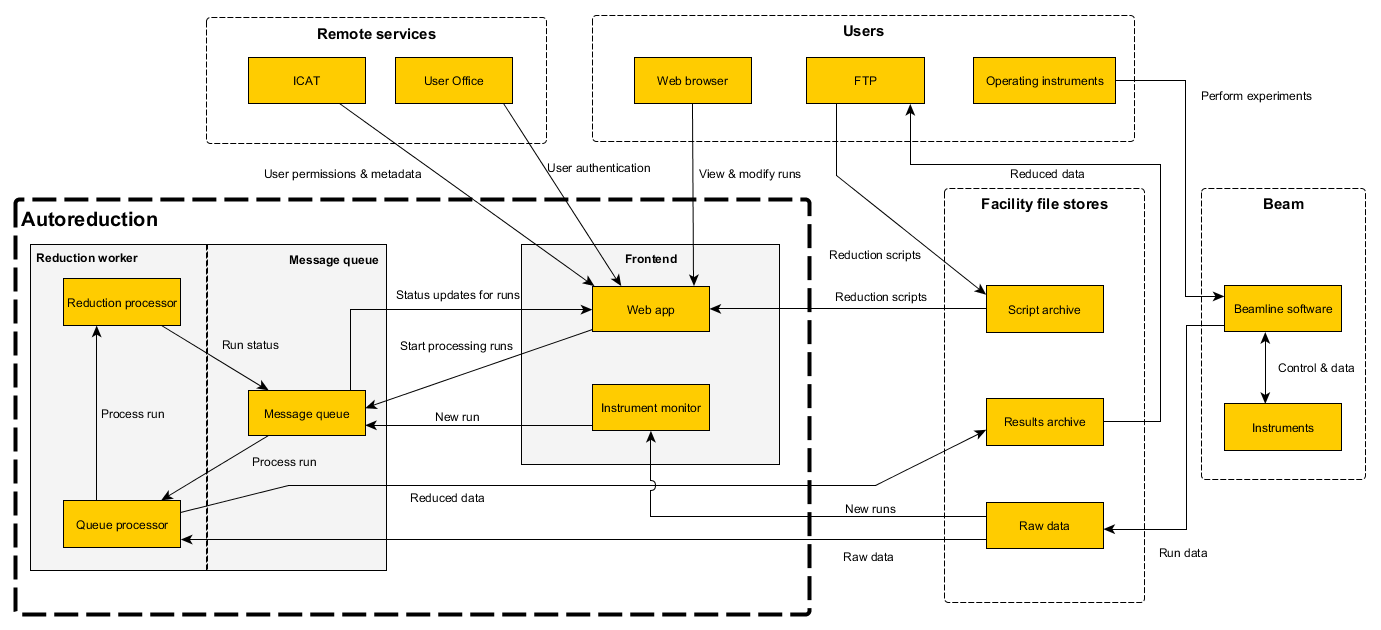
\includegraphics[width=1.15\linewidth,angle=90,origin=c]{system.png}
\caption{How the autoreduction system fits into the ISIS workflow.}
\end{figure*}

\subsection{Message queue}\label{message-queue}

Apache ActiveMQ\cite{activemq} is used as the message queueing system, with
message contents as JSON-formatted objects. The intention of the message
is conveyed by which queue it's placed in, rather than a field in the
message itself. Runs can be `scheduled' simply by using ActiveMQ's
scheduled delay feature, which allows a message to be delivered a given
time after it's been pushed to the queue.

Messages contain metadata for the run such as a (unique) run number and
version, the experiment and instrument that the data is associated with,
and any logs or errors resulting from reduction. They also carry the
necessary information to carry out the data reduction - the Python
script to run on the data, paths to the data, and variables to be used
by the script.

Data files typically run in the hundreds of MB at least, so would be
impractical to send directly in a message; they're provided as file
paths on a shared file archive. Meanwhile, the reduction script to be
used is sent as a string; the script is served from the state database,
and using the message queue directly to send it obviates the need to
rely on a potentially flaky shared file store within the system.

\subsection{Job listener}\label{job-listener}

When a new run has been completed on the beam line, the data files are
placed in a shared filesystem. A node runs a Python watchdog daemon that
tracks changes in this filesystem, and when a new run is added, sends a
message to \emph{Data Ready} with details of the run. This particular
choice of listener isn't crucial; anything would work as long as it
pushed the same message to the queue. In the current production system
at ISIS, this is the same node as the state database itself.

\subsection{State database}\label{state-database}

A node keeps track of the status of runs in a local SQL database. This
server hosts a Python service responsible for listening on \emph{Data
Ready}, to create new runs and then dispatch them to \emph{Reduction
Pending}. It manages variables for reduction, and selects the correct
set for the run. The same server is responsible for serving the
Python/Django\cite{django} web app. The database is therefore accessed through
Django's object interface, and reduction runs, etc., are tracked as
Django objects.

The daemon receives status updates from reduction workers on
\emph{Reduction Started}, \emph{Reduction Complete} and \emph{Reduction
Error}, making the appropriate changes to the database. On some messages
in the error queue, the daemon will create and schedule the appropriate
retry runs. A system for emailing notifications of run failures to
administrators is also implemented here.

\subsection{Reduction worker}\label{reduction-worker}

The data reduction itself is performed by a worker node, running a
Python daemon listening on \emph{Reduction Pending}. When the worker
consumes a message, it will spawn a process starting the job and
notifying \emph{Reduction Started}. This process tests for access to the
filesystems used for storing the raw and reduced data, triggering a
scheduled retry later -- on \emph{Reduction Error} -- if they're
unavailable. Otherwise, it will proceed with the reduction, loading and
then running the provided script.

On a successful run, the job will notify \emph{Reduction Completed} with
the location of the reduced data; otherwise, it will send the reason for
failure to \emph{Reduction Error}, most likely without triggering a
retry. In both cases it will send logs of the process, and clean up
after itself. Some runs associated with the same experiment would write
output to the same directory; to prevent clashes due to this, the node
contains an internal queue holding all runs associated with an
experiment for as long as it's actively reducing another run for the
same experiment.


\begin{figure*}
\centering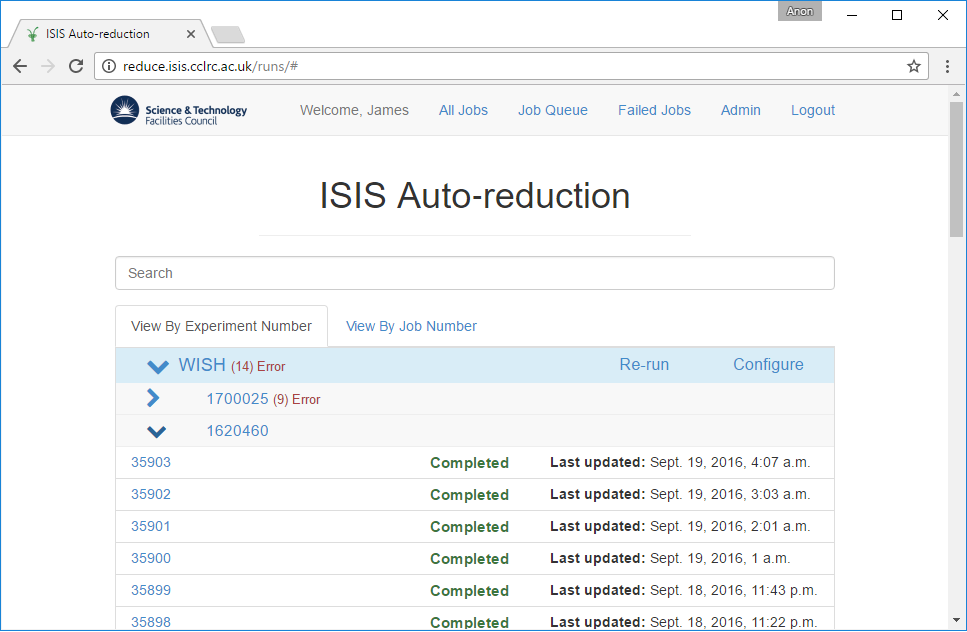
\includegraphics[width=0.8\linewidth]{index.png}
\caption{The web app index, showing recent runs.}
\end{figure*}

\section{Interface}\label{interface}

\subsection{Reduction scripts}\label{reduction-scripts}

The wholly automated portion of the system revolves around running
scientist-provided scripts to reduce raw instrument data. These scripts
are provided as Python scripts on a per-instrument basis, typically
using the Mantid software package to do the heavy lifting. They're
stored on a shared file store in a known location, where they can be
modified at will by instrument scientists; runs store the script they
were reduced by in the system database, but new runs will be reduced
using the current script on the file store.

Aside from overall logic, these scripts typically require parameters
such as calibration files, information about how the instrument was run,
output settings, and so on. While some users prefer to hard-code these
in their scripts, others would rather make use of a system for managing
these variables separate from the script itself. A list of variables and
default values is provided in a Python file similar to the reduction
script, but the autoreduction system keeps track of variable
configurations provided to it through the web app, and applies them to
the relevant runs.

The reduction scripts need to integrate with the automation system, and
as such must conform to a certain specification: the script must have a
\emph{main()} method, taking an input file and an output directory as
arguments. If the script uses system-supplied variables, it must have a
certain \emph{import} directive, which serves as a point of injection
for the variables when it is run.

Mantid provides a wrapper for data reduction through its Python
interface, and for many instruments the whole reduction processing is
also included. Writing reduction scripts for those instruments is
essentially trivial, boiling down to some boilerplate with very little
difference between instruments.

\subsection{Web app}\label{web-app}

The web app provides the user-facing interface for managing reduction.
It was developed in Python, using the Django web framework, and is
tightly integrated with the state database.

Users log in via the ISIS User Office system -- using credentials 
granted for facility-wide use -- and their level of access is then 
governed by ICAT's information on the experiments and instruments they 
should be able to see. A searchable index of runs is displayed on the front page, sorted
by instrument, experiment and run number, showing their reduction
status. Runs, experiments and instruments displayed here have links to
their summary pages.

Each run has its own summary page with detailed information; a user can
see the status of the reduction, where the reduced data is, and the
script and variables that were used to reduce it. From here the run can
be re-run, with or without modifying the variables used. Any
experimenter can access this page for their runs, and it's intended that
external scientists running experiments be able to control their data
reduction directly in this way.

Experiments also have summary pages, showing all the runs that are
associated with a given experiment along with their status and data
locations. Metadata about the experiment is retrieved from ICAT and
displayed here.

Instrument scientists can access a summary page for their instruments,
showing the current status of runs on an instrument, as well as current
and upcoming run variables. From here instrument scientists can assign
sets of variables by experiment and run number, which will then be used
automatically as appropriate for new runs. Batch re-running of past jobs
is also possible here. This is intended to be the main point of access
for instrument scientists to control data reduction.

Administrators can access everything above, and additionally have access
to pages displaying all queued and failed jobs. These pages provide an
overview of the status of the system at a glance, and have controls for
batch operations on failed jobs such as to re-run them.

\section{Current status}\label{current-status}

The system is deployed at ISIS, in limited use. The frontend node,
serving the message queue as well as managing the state and web app, is
a Windows Server system running on a Hyper-V\cite{hyper-v} virtualisation
cluster; it serves the web app using Microsoft's Internet Information
Services (IIS)\cite{iis} and FastCGI\cite{fcgi}. There is one reduction node, 
running Red Hat Enterprise Linux 7\cite{rhel} on a dedicated server -- 
reducing large amounts of data is very CPU-intensive.

It is planned that the autoreduction system be developed to further meet
the needs and tastes of potential users at ISIS and other particle
facilities, and enter a more prominent role in automating data
processing there. Future development to this end may involve

\begin{enumerate}
\item
  Expanding the system to accommodate greater volume of use -- this
  might involve adding more reduction workers, for example.
\item
  Integrating other methods of listening for new runs -- the current
  method of watching a file archive is specific to ISIS.
\item
  Improving portability and deployability of the current software; the
  state database/webapp in particular is currently unsupported for
  Linux, and the whole system is somewhat nontrivial to deploy even to a
  development environment.
\end{enumerate}

\section{Conclusion}\label{conclusion}

The autoreduction system offers a convenient way of automating data reduction
on beamline instruments. It uses a scalable architecture to allow prompt
reduction of data from a large number of instruments, and utilises a web app
frontend to allow users to control the reduction process manually and verify
that the correct reduction was run.

The system is currently in limited use at ISIS, with more instrument scientists
interested in using it. The source code can be found on GitHub\cite{source}.

\begin{thebibliography}{99}
\bibitem{mantid}
    O. Arnold, et al.,
    \emph{Mantid -- Data analysis and visualization package for neutron scattering and $\mu$SR experiments},
    Nuclear Instruments and Methods in Physics Research Section A, Volume 764, 11 November 2014, Pages 156-166,
    \href{http://dx.doi.org/10.1016/j.nima.2014.07.029}{10.1016/j.nima.2014.07.029}.
    
\bibitem{icat}
    The ICAT Collaboration,
    \emph{The Icat Project.},
    2014,
    \href{https://doi.org/10.5286/SOFTWARE/ICAT}{10.5286/software/icat}.
    
\bibitem{activemq}
    Apache Software Foundation,
    \emph{Apache Activemq},
    \url{http://activemq.apache.org/}.
    
\bibitem{django}
    Django Software Foundation,
    \emph{Django},
    \url{https://www.djangoproject.com/}.
    
\bibitem{hyper-v}
    Microsoft Corporation,
    \emph{Hyper-V},
    \url{https://technet.microsoft.com/en-us/library/mt169373.aspx}.
    
\bibitem{iis}
    Microsoft Corporation,
    \emph{IIS},
    \url{http://www.iis.net/}.
    
\bibitem{fcgi}
    \emph{FastCGI},
    \url{https://github.com/FastCGI-Archives/FastCGI.com}.
    
\bibitem{rhel}
    Red Hat, Inc,
    \emph{Red Hat Enterprise Linux},
    \url{https://www.redhat.com/en/technologies/linux-platforms/enterprise-linux}.
    
\bibitem{source}
    \emph{Autoreduction repository},
    \url{https://github.com/mantidproject/autoreduce}.

    
\end{thebibliography}
\end{document}
